% Options for packages loaded elsewhere
\PassOptionsToPackage{unicode}{hyperref}
\PassOptionsToPackage{hyphens}{url}
%
\documentclass[
]{article}
\usepackage{lmodern}
\usepackage{amssymb,amsmath}
\usepackage{ifxetex,ifluatex}
\ifnum 0\ifxetex 1\fi\ifluatex 1\fi=0 % if pdftex
  \usepackage[T1]{fontenc}
  \usepackage[utf8]{inputenc}
  \usepackage{textcomp} % provide euro and other symbols
\else % if luatex or xetex
  \usepackage{unicode-math}
  \defaultfontfeatures{Scale=MatchLowercase}
  \defaultfontfeatures[\rmfamily]{Ligatures=TeX,Scale=1}
\fi
% Use upquote if available, for straight quotes in verbatim environments
\IfFileExists{upquote.sty}{\usepackage{upquote}}{}
\IfFileExists{microtype.sty}{% use microtype if available
  \usepackage[]{microtype}
  \UseMicrotypeSet[protrusion]{basicmath} % disable protrusion for tt fonts
}{}
\makeatletter
\@ifundefined{KOMAClassName}{% if non-KOMA class
  \IfFileExists{parskip.sty}{%
    \usepackage{parskip}
  }{% else
    \setlength{\parindent}{0pt}
    \setlength{\parskip}{6pt plus 2pt minus 1pt}}
}{% if KOMA class
  \KOMAoptions{parskip=half}}
\makeatother
\usepackage{xcolor}
\IfFileExists{xurl.sty}{\usepackage{xurl}}{} % add URL line breaks if available
\IfFileExists{bookmark.sty}{\usepackage{bookmark}}{\usepackage{hyperref}}
\hypersetup{
  pdftitle={Impact of Price on AirBnb Bookings in Los Angeles},
  pdfauthor={Austin Jin, Lynn Marciano, Jacquie Nesbitt, Huyette Spring},
  hidelinks,
  pdfcreator={LaTeX via pandoc}}
\urlstyle{same} % disable monospaced font for URLs
\usepackage[margin=1in]{geometry}
\usepackage{longtable,booktabs}
% Correct order of tables after \paragraph or \subparagraph
\usepackage{etoolbox}
\makeatletter
\patchcmd\longtable{\par}{\if@noskipsec\mbox{}\fi\par}{}{}
\makeatother
% Allow footnotes in longtable head/foot
\IfFileExists{footnotehyper.sty}{\usepackage{footnotehyper}}{\usepackage{footnote}}
\makesavenoteenv{longtable}
\usepackage{graphicx,grffile}
\makeatletter
\def\maxwidth{\ifdim\Gin@nat@width>\linewidth\linewidth\else\Gin@nat@width\fi}
\def\maxheight{\ifdim\Gin@nat@height>\textheight\textheight\else\Gin@nat@height\fi}
\makeatother
% Scale images if necessary, so that they will not overflow the page
% margins by default, and it is still possible to overwrite the defaults
% using explicit options in \includegraphics[width, height, ...]{}
\setkeys{Gin}{width=\maxwidth,height=\maxheight,keepaspectratio}
% Set default figure placement to htbp
\makeatletter
\def\fps@figure{htbp}
\makeatother
\setlength{\emergencystretch}{3em} % prevent overfull lines
\providecommand{\tightlist}{%
  \setlength{\itemsep}{0pt}\setlength{\parskip}{0pt}}
\setcounter{secnumdepth}{5}

\title{Impact of Price on AirBnb Bookings in Los Angeles}
\usepackage{etoolbox}
\makeatletter
\providecommand{\subtitle}[1]{% add subtitle to \maketitle
  \apptocmd{\@title}{\par {\large #1 \par}}{}{}
}
\makeatother
\subtitle{What can the Los Angeles Tourism \& Convention Board learn about AirBnb booking behavior?}
\author{Austin Jin, Lynn Marciano, Jacquie Nesbitt, Huyette Spring}
\date{}

\begin{document}
\maketitle

{
\setcounter{tocdepth}{2}
\tableofcontents
}
\clearpage

\hypertarget{introduction}{%
\section{Introduction}\label{introduction}}

Throughout the year 2020, tourism and hospitality industries throughout the world have been tremendously impacted by the COVID-19 pandemic. Government bodies, healthcare workers, and even celebrities urged people in Los Angeles to ``stay home and stay strong'' in order to prevent the spread of the contagious virus. Now, more than a year later, over 300 vaccine projects have commenced and conducted a series of undergoing evaluations to eventually introduce viable vaccines that passed Phase III clinical trials into the United States market, specifically from top pharmaceutical corporations such as Pfizer, Johnson \& Johnson, and Moderna. Even with some reluctance for vaccinations that stems from mistrust and medical disenfranchisement, more than half of U.S. citizens have been vaccinated, and over 70\% of those aged 16+ years old have received at least 1 dose within the county of Los Angeles.

With that being said, there have been confirmed studies of major reductions in SARS-CoV-2 infections amongst those receiving doses of the COVID-19 vaccine which led to airlines reopening on a massive scale. Also ``revenge travel'', which is the concept that people are now more eager to travel after a year of putting trips on hold, has hence become a frequently used phrase in our current vocabularies. City dwellers seeking to escape their COVID-19 refuges are road-tripping to nearby vacation rentals in staggering numbers, showing the first signs of life for an industry that essentially ground to a halt since March of last year. Knowing that people are now more eager than ever to revisit open spaces with Mediterranean climates and beach towns such as Southern California, we have decided to study the elements that drive higher motivation to travel during these times as part of the data science team for the Los Angeles Tourism \& Convention Board. In essence, our data science team will be aiming to maximize Los Angeles County's tourism industry throughout this period of higher motivation to travel.

To provide some context as to the reasons behind narrowing down our scope into a single county, Los Angeles has in particular seen continuous breakthroughs of coronavirus cases and hospitalizations for the recent months even with vaccinations being introduced to the state. It became obvious for our team to dig deeper into the situation's impact on tourism and hospitality knowing that the county would still be placed in the most restrictive purple tier bracket if tier-based blueprints were still in place for lifting coronavirus restrictions. Despite the county's unending surge in hospitalized COVID-19 patients and deaths, there have been increasing rates of travel to Los Angeles due to being one of the most popular tourism destinations in the United States, which ultimately leads to increases in bookings through accommodation rental services such as Airbnb and hotels. We have, however, decided to specifically focus on Airbnb over other accommodation providers to help our fellow Los Angeles residents recoup some of the financial losses throughout the past year.

By understanding factors that lead people to make booking decisions, our team would be able to provide better guidance to Los Angeles's tourism and hospitality industries to capitalize on higher interest. To further prepare for the upward trend in bookings, our research study will focus on finding the components that contribute to booking 60 days out through Airbnb. More specifically, our team has decided to analyze the relationship between Airbnb prices and the number of bookings within Los Angeles County to answer the following research question:

\textbf{How does price affect Airbnb bookings?}

Through our analysis, we will be establishing whether Airbnb prices impact bookings to provide insights into the determinants that travelers use to finalize booking decisions. We hope to utilize our results to better inform the Los Angeles Tourism \& Convention Board on whether prices and other interaction variables are a factor in the increases in Airbnb bookings so that we could ultimately increase Los Angeles resident's income through tourism.

\hypertarget{model-building-process}{%
\section{Model Building Process}\label{model-building-process}}

\hypertarget{data-description}{%
\subsection{Data Description}\label{data-description}}

Data Source: \href{http://insideairbnb.com/get-the-data.html}{Inside Airbnb Listings Data}
\href{https://docs.google.com/spreadsheets/d/1iWCNJcSutYqpULSQHlNyGInUvHg2BoUGoNRIGa6Szc4/edit\#gid=0}{Data Dictionary}

To operationalize our research question, we utilized data from Inside Airbnb. Inside Airbnb scrapes publicly available information about a city or county's Airbnb listings. The accuracy of the information compiled from the Airbnb site is not controlled by Inside Airbnb. However, Inside Airbnb has analyzed, cleansed, and aggregated the compiled data where appropriate.

It is important to note that Inside Airbnb is an advocacy group that advocates for reducing Airbnb short-term rentals. Although ``due care'' has been taken with the processing and analysis of the dataset, we remain cautious about the cleanliness and objectivity of this data, the advocacy group's motivation for collecting this data, and the risk of listings being removed after data cleansing.

We have chosen this specific dataset to combat the financial losses of our fellow Los Angeles citizens as well as to prepare for the increases in ``revenge travel'' now that most travel restrictions have been lifted. Due to our motives in the Los Angeles Tourism \& Convention Board, we hope that by understanding how price affects Airbnb bookings we can gain insight on how to increase the levels of tourism again in Los Angeles County.

\hypertarget{exploratory-data-analysis}{%
\subsection{Exploratory Data Analysis}\label{exploratory-data-analysis}}

Based on our step-by-step assumptions on the key motive variables that would lead individuals to book a listing on Airbnb, we have decided to utilize the following variables for our analysis:

\begin{itemize}
\item
  availability\_60
\item
  price
\item
  Room\_type
\item
  reviews\_scores\_rating
\item
  accommodates
\item
  instant\_bookable
\end{itemize}

\textbf{Filtering}

When assessing our variables, we wanted to define who a vacationer would be. Typically individuals will book for a short period of time when vacationing. However, we found listings where the minimum number of nights for a booking was greater than 60 days. This led us to assume that these listings may be used more so for rental purposes rather than vacationing. We decided to filter our data to remove listings with more than a 60 day minimum booking. It is also worth mentioning that travelers usually traveled for 2 weeks or more but now with COVID-19 reshaping the travel industry, travelers are working remote and staying in places longer than usual. Thus, we have decided to remove all listings that did not fit this criteria.

Furthermore, when looking at the ``availability\_60'' variable and ``has\_availability'' variable, we noticed a discrepancy between the two. The ``has\_availability'' variable states where there is availability for booking the listing. However, we found that the ``availability\_60'' and the other ``availability\_n'' would be 0, which states there is no availability, and the listing is fully booked. We decided to remove the rows where we found this discrepancy.

\textbf{availability\_60}

The ``availability\_60'' variable represents the availability of the listing 60 days into the future as determined by the calendar from the data scrape date. Although there were other ``availability\_x'' variables, we decided to focus on two months out from the calendar scrape date. We recognize peak tourism season is between June to August; with our data being scrapped at the beginning of July, we felt that assessing the middle of peak tourism season would be insightful towards our goals. The less availability a listing has, the more bookings it receives. It is important to note that a listing may not be available due to being booked by a guest or blocked by the host.

When assessing the variable, we notice that it is multimodal. This led to our assumption that the availability among listings fluctuates during the tourism season.

\textbf{price}

The ``price'' variable represents the daily price for the listing, assuming that the price will be the same for all the days in the calendar dates. The variable also does not include any additional charges that are included when booking a listing, such as: cleaning fees, booking fees, pet fees, etc. We wanted to focus our research on price because we believe that price is the most important motive when individuals book a listing on Airbnb.

When assessing the ``price'' variable, we observed that it is right-skewed. This confirms our assumptions that listings are typically moderately priced and only few are abnormally priced higher than the average. Applying a base10 log transform to the variable makes it normally distributed for our statistical analysis.

\textbf{room\_type}

The ``room\_type'' variable represents the type of listing grouped into the following categories:

\begin{itemize}
\item
  Entire place
\item
  Private room
\item
  Hotel room
\item
  Shared room
\end{itemize}

Based on our assumptions, individuals, who are vacationing, will typically prefer a listing that is more private. Furthermore, with the effects of the COVID-19 pandemic, we assume individuals would feel more comfortable having their own space. Entire places may be more sought after due to having the whole space to yourself. With private rooms, an individual still has some of their own space but may share corridors with others, such as the host, or other travelers. Private rooms are typically more affordable than entire spaces, so an individual may choose this option over the latter. A Shared Room is where the individual will be sleeping in a shared space with others. Based on our hypothesis of social awareness from the pandemic, we assessed this listing would not likely be highly represented in our dataset. Hotel Rooms offer a private space similar to that of an Airbnb private room but with the convenience of online booking for most hotels, it is more likely that an individual would book on platforms other than Airbnb.

\textbf{reviews\_scores\_rating}

The ``reviews\_scores\_rating'' variable represents the ratings score for listings from 0 (worst) to 5 (best) for the overall experience and for specific categories, including: overall experience, cleanliness, accuracy, value, communication, check-in, and location. The host would need to get at least 3 star ratings in order for the overall rating to appear on the listing or profile. We felt this variable was important as a motive behind booking on Airbnb due to the assumption that individuals would want a quality stay when traveling.

When assessing the variable, we observed that it is left-skewed. It was in fact our heaviest skewed variable. Transforms such as log and poly-normalizing the variable showed no effect. This led us to assume that every coefficient in the variable was significant. However, a rating from 1-2 is not the same as 4-5 due to the subjective nature of individuals based on their experience during their stay.

When assessing the relationship between price, rating and room\_type. We were able to observe that private stays, such as, ``Entire homes/apartments'', ``Hotel Rooms'', and ``Private Rooms'' were indeed priced higher than ``Shared Rooms''. Many of the listings are clustered around higher ratings; however, there is a linear declination in price when the ratings are higher. This led us to assume that listings with better ratings could be a result of being valued at a better price.

\textbf{accommodates}

The ``accommodates'' variable represents the maximum capacity of the listing. In order words, the variable provided us with data on the number of guests that could be housed for the given listing. We recognized this variable as a criterion when booking an Airbnb reservation and intended on seeking whether there was any relationship between accommodations coupled with price and room type with the availability of the listing 60 days out.

When observing the distribution of the capacity of Airbnb bookings, we notice that it was right-skewed. This led to our assumption that most listings are capable of hosting 8 or fewer guests and there are very few listings that are able to accommodate more.

\textbf{instant\_bookable}

The ``instant\_bookable'' represents whether the guest can automatically book the listing without the host being required to accept their booking request. This variable was considered an indicator of a commercial listing. It is also worth mentioning that ``instant\_bookable'' is a boolean data type in that ``t'' would equal true for the guest being able to automatically book the listing without host approvals and ``f'' for the guest not being able to automatically book the listing without host approvals.

We felt this variable would be important to include in our models due to the convenient nature of humans' daily lives. We wanted to see if the convenience factor of being able to instantly book a listing without discussing with a host would increase the likelihood of a listing being booked. When assessing the listings that were instant-bookable, we observed that more listings were not instant-bookable. This led to our assumption that most listings on Airbnb are privately owned, rather than commercially owned.

\hypertarget{model-selection-and-the-subset-selections}{%
\subsection{Model Selection and the Subset Selections}\label{model-selection-and-the-subset-selections}}

Our models were structured under the notion of assumptions that would motivate individuals to book certain Airbnbs. The general framework considered thinking patterns that would drive motivations for individuals to book on Airbnb. Individual motivations also included the built-in features that the Airbnb platform has to offer. Below is a brief explanation for all 4 models:

\textbf{Model 1}

Model 1 is our limited model that assesses the relationship between our key variable ``price'' and ``availability\_60''. In essence, we intended to measure how price affects bookings that are 60 days out into the future. Before applying any transformations, price was right-skewed. We applied a base10 log transformation to the variable and the distribution became normal.

\textbf{Model 2}

Model 2 includes some additional explanatory variables that we believed were other motives for booking through Airbnb. We assumed that the type of listing (``room\_type'') and rating (``reivews\_scores\_rating'') was part of the primary framework when an individual performed bookings on Airbnb.

\textbf{Model 3}

Model 3 includes another covariate that we believed would be part of the booking process. Knowing that the size of a booking party is considered an important criteria when filtering results through Airbnb, we have decided to add in the ``accommodates'' variable for specific bookings that are based on the accommodation capacity of a listing.

\textbf{Model 4}

Model 4 includes another covariate that we believed would drive more bookings. Knowing that individuals prefer convenience when it comes to being able to seamlessly book through an online platform, we have decided to also include the ``instant\_bookable'' variable as a factor that would affect the number of bookings.

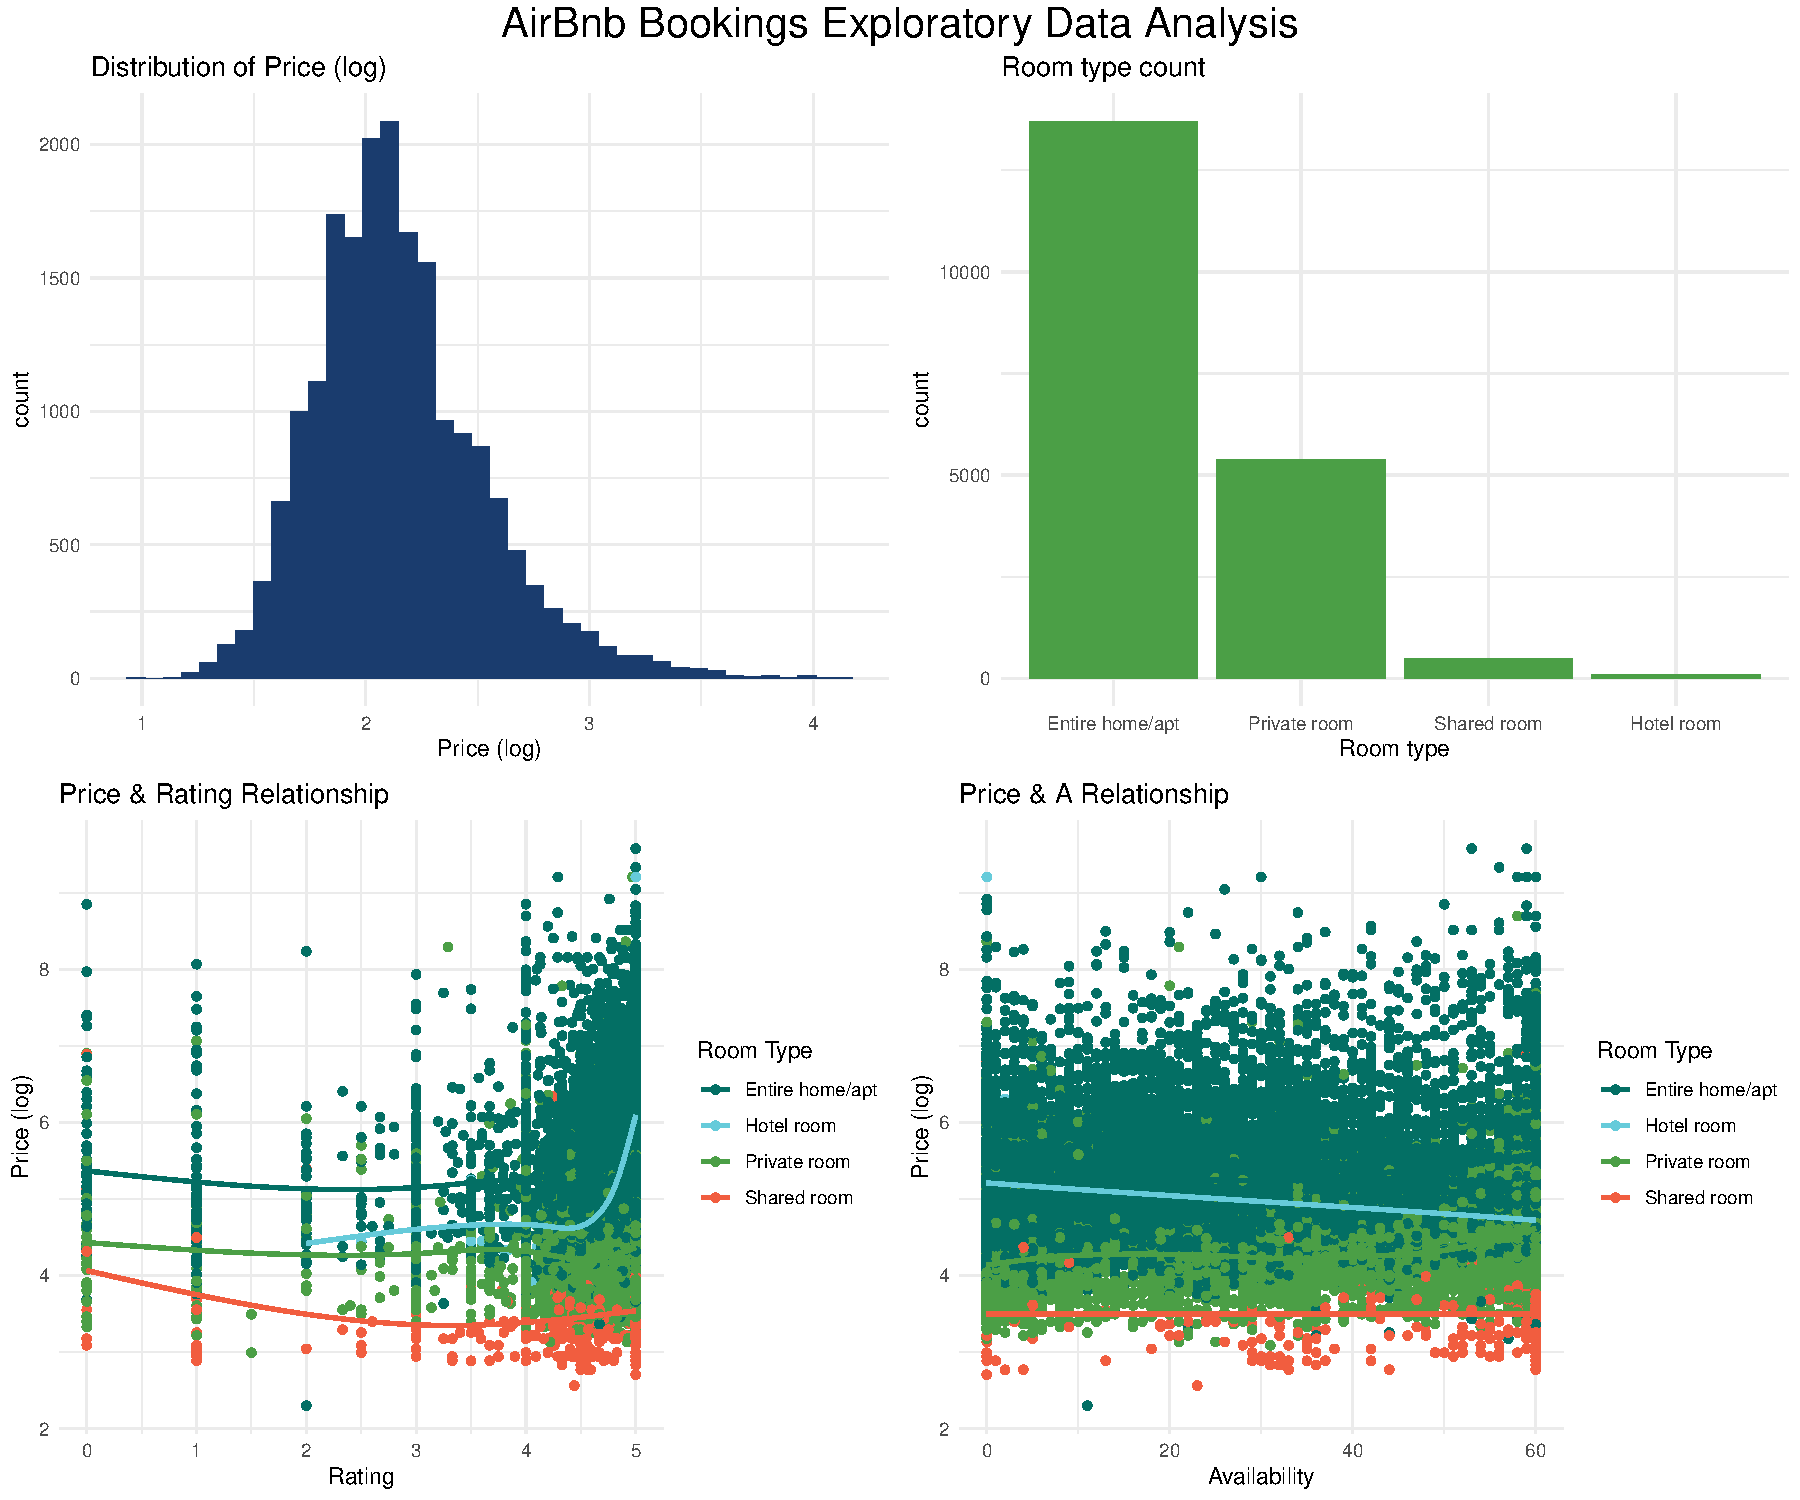
\includegraphics{lab2_report_files/figure-latex/eda_charts-1.pdf}

\hypertarget{regression-results}{%
\section{Regression Results}\label{regression-results}}

\begin{verbatim}
## 
## Regression Results with Standard Robust Errors
## ====================================================================================================================================================
##                                                                                      Dependent variable:                                            
##                                           ----------------------------------------------------------------------------------------------------------
##                                                                               Availability 60 days In The Future                                    
##                                                  Price Only           + Room Type and Rating         + Accommodates          + Instantly Bookable   
##                                                      (1)                       (2)                        (3)                        (4)            
## ----------------------------------------------------------------------------------------------------------------------------------------------------
## Log of Price                                  2.665*** (0.405)          11.711*** (0.458)          14.583*** (0.606)          14.678*** (0.606)     
## Hotel Room                                                              19.529*** (2.833)          18.616*** (2.874)          17.343*** (2.877)     
## Private Room                                                            10.079*** (0.386)           9.732*** (0.386)           9.805*** (0.386)     
## Shared Room                                                             31.047*** (1.014)          31.814*** (1.041)          31.543*** (1.035)     
## Overall Rating                                                          -4.159*** (0.271)          -4.238*** (0.273)          -4.144*** (0.272)     
## Number of People the Listing Accommodates                                                          -0.653*** (0.077)          -0.665*** (0.077)     
## Instantly Bookable                                                                                                             2.036*** (0.291)     
## Constant                                      20.161*** (0.894)         16.620*** (1.667)          13.293*** (1.738)          12.015*** (1.749)     
## ----------------------------------------------------------------------------------------------------------------------------------------------------
## Observations                                       19,647                     19,647                     19,647                     19,647          
## R2                                                  0.002                     0.094                      0.098                      0.100           
## Adjusted R2                                         0.002                     0.094                      0.097                      0.100           
## Residual Std. Error                          20.458 (df = 19645)       19.495 (df = 19641)        19.459 (df = 19640)        19.436 (df = 19639)    
## F Statistic                               47.730*** (df = 1; 19645) 409.265*** (df = 5; 19641) 354.570*** (df = 6; 19640) 311.308*** (df = 7; 19639)
## ====================================================================================================================================================
## Note:                                                                                                                    *p<0.1; **p<0.05; ***p<0.01
\end{verbatim}

According to the regression results, one thing that stands out is that all variables are statistically significant and the coefficients are somewhat stable across model 2, model 3, and model 4. Overall, the main takeaway from these regressions is that our models do find a statistically significant relationship between price and a listing's availability 60 days into the future. However, given the severe violations to I.I.D and linear conditional expectation assumptions, we cannot trust our regression coefficients, and given the violations to the normally distributed assumptions, we cannot trust our hypothesis testing results. Therefore we cannot trust these regression models.

Across models 2, 3, and 4, we believe Model 4 is the one that would best capture potential effects because of its higher adjusted R-squared as compared to the other model specifications, additionally, we ran ANOVA which determined that each model was statistically significant compared to its predecessor. That being said, due to the recursive nature of the booking behavior we considered a more complex model which includes interaction terms. While this model boosted the adjusted R-squared and the variable of interest was less by 1 day than the non-interaction model, we did not feel the additional complexity was worth it, especially in light of the low adjusted R-squared, its interpretation complexity, and it didn't help meet the CLM assumptions.

\begin{verbatim}
## Analysis of Variance Table
## 
## Model 1: availability_60 ~ log10(price)
## Model 2: availability_60 ~ log10(price) + factor(room_type) + review_scores_rating
## Model 3: availability_60 ~ log10(price) + factor(room_type) + review_scores_rating + 
##     accommodates
## Model 4: availability_60 ~ log10(price) + factor(room_type) + review_scores_rating + 
##     accommodates + instant_bookable
##   Res.Df     RSS Df Sum of Sq       F    Pr(>F)    
## 1  19645 8222353                                   
## 2  19641 7464619  4    757735 501.447 < 2.2e-16 ***
## 3  19640 7436773  1     27845  73.709 < 2.2e-16 ***
## 4  19639 7419103  1     17670  46.775 8.198e-12 ***
## ---
## Signif. codes:  0 '***' 0.001 '**' 0.01 '*' 0.05 '.' 0.1 ' ' 1
\end{verbatim}

\hypertarget{clm-assumptions-and-limitations-of-the-model}{%
\section{CLM Assumptions and Limitations of the Model}\label{clm-assumptions-and-limitations-of-the-model}}

Given the number of observations in the dataset (31,543), we believe it is reasonable to rely on the Central Limit Theorem. However, for the purposes of articulating the limitations of our model, we evaluate the five Classic Linear Model assumptions. As demonstrated below, our model fails a number of these tests, providing justification for the use of Robust Standard Errors.

\hypertarget{iid-sampling}{%
\subsection{\texorpdfstring{\textbf{1. IID Sampling}}{1. IID Sampling}}\label{iid-sampling}}

There are several characteristics of the data to note when evaluating IID.

\textbf{Inside Airbnb is an advocacy group.} While Inside Airbnb may not have altered the data, there is no way to validate this. At a minimum, we relied on this advocacy to provide the cleaned data from the scraping process. Accordingly, we must assume that the data has some degree of bias, violating the assumption of IID, albeit to an unknown degree.

\textbf{Supply / Demand Recursion.} Airbnb is a marketplace, balancing supply and demand through price. In this marketplace, landlords compete to have their rooms booked. By definition, the price and availability of one room will impact the price and availability of another, in a recursive loop characteristic of all markets. Therefore, while the data only represents a point in time (as opposed to a time-based study), the nature of the data violates a core assumption of IID sampling, namely, independence.

\textbf{Geography.} As representatives of the Los Angeles Tourism Department, we are focused on the City of Los Angeles, specifically. While this is a reasonable and practical approach for the study, it does not represent random sampling. The renter and rentee behaviors within Los Angeles, or even within neighborhoods in Los Angeles, are unlikely to be truly independent from one another. While potentially unavoidable, this does limit the assumption of IID.

Based on the above, we make specific note of the limitations of the IID assumption for this dataset. However, we also note that it may be nearly impossible, and at a minimum impractical, to remove these limitations. Accordingly, for the purposes of this study, we proceed under the assumption that the data is IID.

\hypertarget{no-perfect-colinearity}{%
\subsection{\texorpdfstring{\textbf{2. No Perfect Colinearity}}{2. No Perfect Colinearity}}\label{no-perfect-colinearity}}

A simple indication of perfect collinearity is that regressions won't run, or will drop a variable.
Based on the Regression Results noted above, we can see that the regression ran appropriately and that no values were dropped (displayed as N/A).
Additionally, running a VIF test did not reveal any scaling values above 5.
Accordingly, we can assume that the model does not include any perfectly collinear variables.

No variables have been dropped when observing the coefficients. There is no perfect collinearity. This assumption also includes that a BLP exists, which may not happen since there are heavy tails for ratings and price.

\hypertarget{linear-conditional-expectation}{%
\subsection{\texorpdfstring{\textbf{3. Linear Conditional Expectation}}{3. Linear Conditional Expectation}}\label{linear-conditional-expectation}}

When assessing the Linear Conditional Expectation, we aim to evaluate whether the data we have can be described in terms of a linear model. If it appears that the residuals are not normally distributed, it may be that, while the model is the best linear predictor, linear relationships cannot fully model the complexity of the data.

We can see here that the distribution of residuals of model3 has a distinct positive skew. Additionally, the ``ocular test'', in which a regression is fit on the scatter plot of prediction against residuals, demonstrates a distinct ``downward swoosh'' in which higher predictions have a significant negative residuals bias. Moreover, the residuals associated with price and review score also notably deviate from zero. This indicates that a model inclusive of polynomial transformations may be more appropriate but is beyond the scope of this study.

Based on the above, we do not believe we have satisfied the assumption of Linear Conditional Expectation.

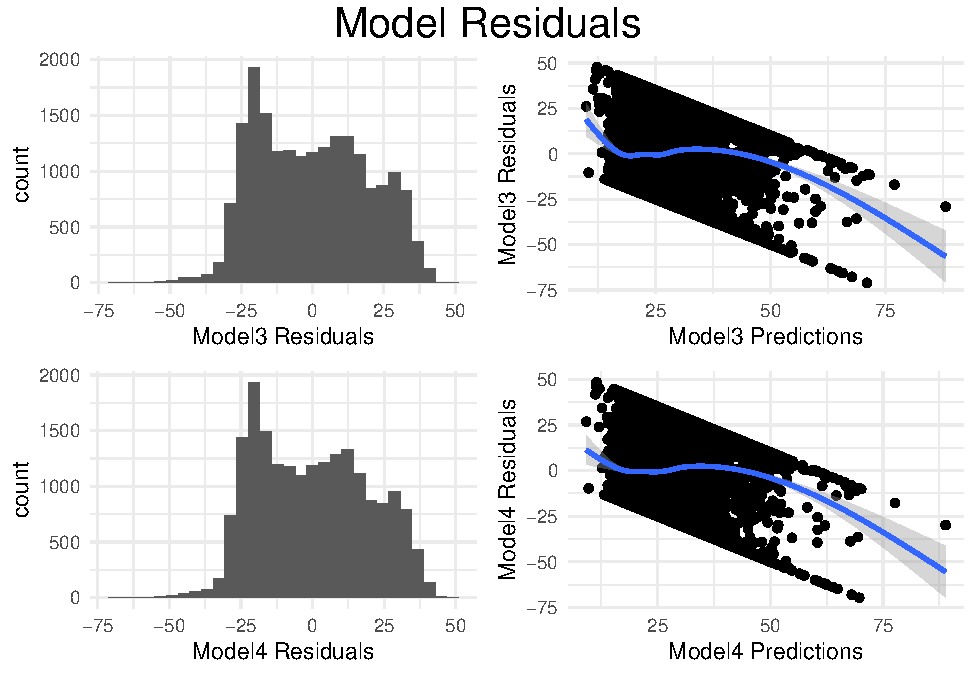
\includegraphics{lab2_report_files/figure-latex/lce_charts-1.pdf}

\hypertarget{homoskedastic-errors}{%
\subsection{\texorpdfstring{\textbf{4. Homoskedastic Errors}}{4. Homoskedastic Errors}}\label{homoskedastic-errors}}

Homoskedastic Error refers to constant, finite conditional error variances. If the conditional error variances differ (Heteroskedastic), it could indicate, mainly, that Classical Standard Errors are biased. Heteroskedastic variance is often caused by, among other things, skewness in the data.
In the case of the Airbnb data, we have already noted the skewness of the data and therefore it is easy to imagine that they have Heteroskedastic variance.

There are two approaches to assessing Homoskedastic Errors: the Breusch-Pagan test, and the ``ocular'' test. As displayed in the Linear Conditional Expectation section above, model3 demonstrates a distinct ``downward swoosh'' in which higher predictions have a significant negative residuals bias.

The ocular test is confirmed by the Breusch-Pagan test which has a materially significant p-value of ​​2.2e-16, suggesting that we reject the null hypothesis of Homoskedacity in favor of Heteroskedasticity.

Based on these tests, we do not believe we have satisfied the assumption of Homoskedastic Errors.

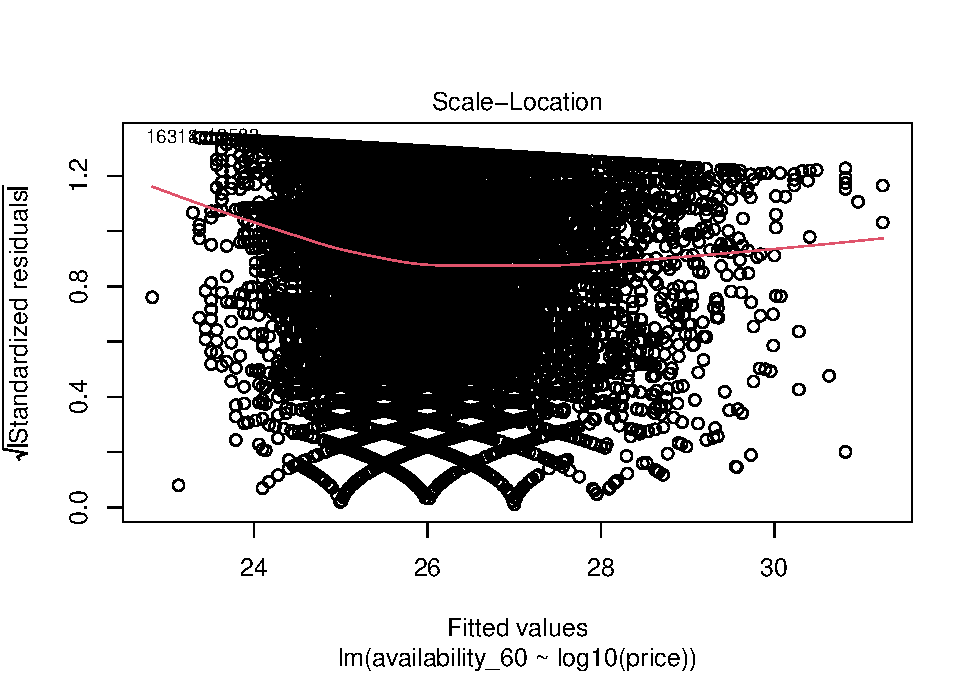
\includegraphics{lab2_report_files/figure-latex/homoskedastic_errors_plots-1.pdf} 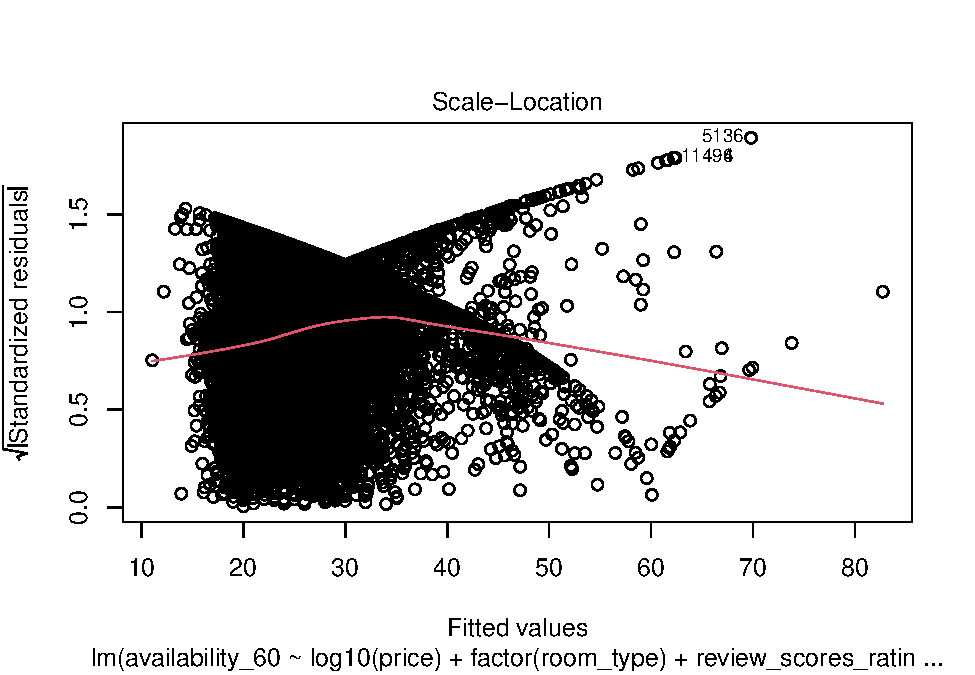
\includegraphics{lab2_report_files/figure-latex/homoskedastic_errors_plots-2.pdf} 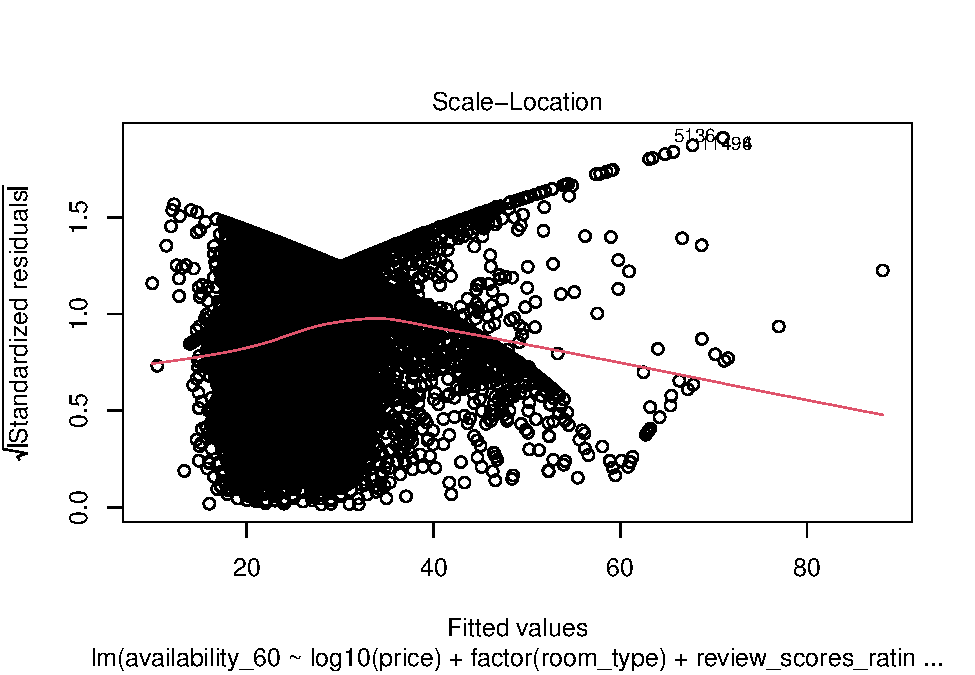
\includegraphics{lab2_report_files/figure-latex/homoskedastic_errors_plots-3.pdf}

\hypertarget{normally-distributed-errors}{%
\subsection{\texorpdfstring{\textbf{5. Normally Distributed Errors}}{5. Normally Distributed Errors}}\label{normally-distributed-errors}}

When evaluating Normally Distributed Errors, we are attempting to demonstrate that the residuals of the model are normally distributed about 0. As can be seen from the histogram above, the distribution of residuals of model3 has a distinct positive skew. Similarly, the Normal Q-Q chart demonstrates material deviations in the Theoretical Quantiles away from the straight-line fit which would indicate a normal distribution.

Again, we believe that the assumption of Normally Distributed Errors has not been met.

\hypertarget{ommitted-variables}{%
\section{Ommitted Variables}\label{ommitted-variables}}

The main relationship we explored in our model was between price and a listing's availability 60 days into the future. As noted above, Airbnb is a marketplace, balancing supply and demand through price in a recursive loop characteristic of all markets. Because of this, identification of Omitted Variables that are not direct outcomes of this recursive balancing of supply and demand is a challenge. In other words, the omitted variables identified must impact availability and price simultaneously rather than influencing one which subsequently influences the other.
Nevertheless, we have attempted to identify such omitted variables below:

\textbf{COVID-19.} In terms of causality, we could easily argue that COVID-19 could cause a decrease in bookings as people stay home. Likewise, we could also argue that it would cause an increase in bookings because people are working remotely and are taking the opportunity to live away from their primary residence longer. We believe this to be a bi-directional variable that could influence the direction of the bias towards or away from zero.

\textbf{Environmental conditions.} We could argue that due to the nearby wildfires happening near Los Angeles the air quality would give potential tourists pause for booking a potential holiday in the area. Therefore we believe this would increase the number of available bookings 60 days out. This implies that the true coefficient of price would be towards zero.

\textbf{General economic conditions.} The general economic conditions of both Los Angeles and the home location of the Airbnb booker could be an omitted variable, biasing availability and price. Positive economic conditions may decrease availability as bookers have more disposable income while also increasing price as landlords anticipate this additional disposable income. Note that, as mentioned above, if landlords increased price as a result of and subsequent to a reduction in supply, this would not be an omitted variable and instead a function of supply and demand balancing through price.

\hypertarget{conclusion}{%
\section{Conclusion}\label{conclusion}}

\textbf{Background and goals.} The group set out to assess the behavior of Airbnb renters with the aim of identifying drivers which the City of Los Angeles may be able to influence to increase tourism in post-COVID.

\textbf{Findings.} We hypothesized that renters evaluate three variables in successive order when evaluating listings:

\begin{itemize}
\item
  Price
\item
  Room type
\item
  Ratings
\end{itemize}

At a high level, our model validated this assumption. We found that price, room type and rates all had a statistically significant impact on booking behavior.

{[}Add in details of the model{]}

\textbf{Next steps.} We encourage the Los Angeles Tourism \& Convention Board to support future research such that this group can identify concrete actions the City of Los Angeles can take to positively impact these variables. This future research may include

\begin{enumerate}
\def\labelenumi{(\roman{enumi})}
\item
  surveys and in-person interviews of both Airbnb renters and rentees to gain a better understanding of actual behavior;
\item
  an enhanced model which captures the findings from these surveys and interviews, potentially including interaction variables; and
\item
  experimental trials to determine the effectiveness of recommended interventions.
\end{enumerate}

\hypertarget{bibliography}{%
\section{Bibliography}\label{bibliography}}

\end{document}
